\section{\uppercase{Best views estimation}}\label{sec:best-views-estimation}

\noindent Estimation of the best views for a constellation of sensors requires both the ability to generate accurate sensor data for each type of sensor and also an efficient approach to compute the surface coverage that we are trying to maximize. The next sections explain how the sensor data is analyzed and also present the approaches used to estimate the best constellation of sensors for a given simulation world.

\subsection{Reference surface point cloud}

The first step in the processing pipeline includes the generation of the multi-object reference point cloud that is built by transforming the point cloud associated with the target \gls{cad} model into each target object within the simulation world (example shown in \cref{fig:reference-cloud}). Later on, the reference point cloud in the world coordinate frame is filtered with a voxel grid algorithm in order to perform a regular space partition and extract the surface voxels centroids that contain points. This approach allows to generate a reference point cloud with a constant surface point density, which will be critical later on when computing the surface coverage percentage achieved with a given sensor constellation.

\begin{figure}
	\centering
	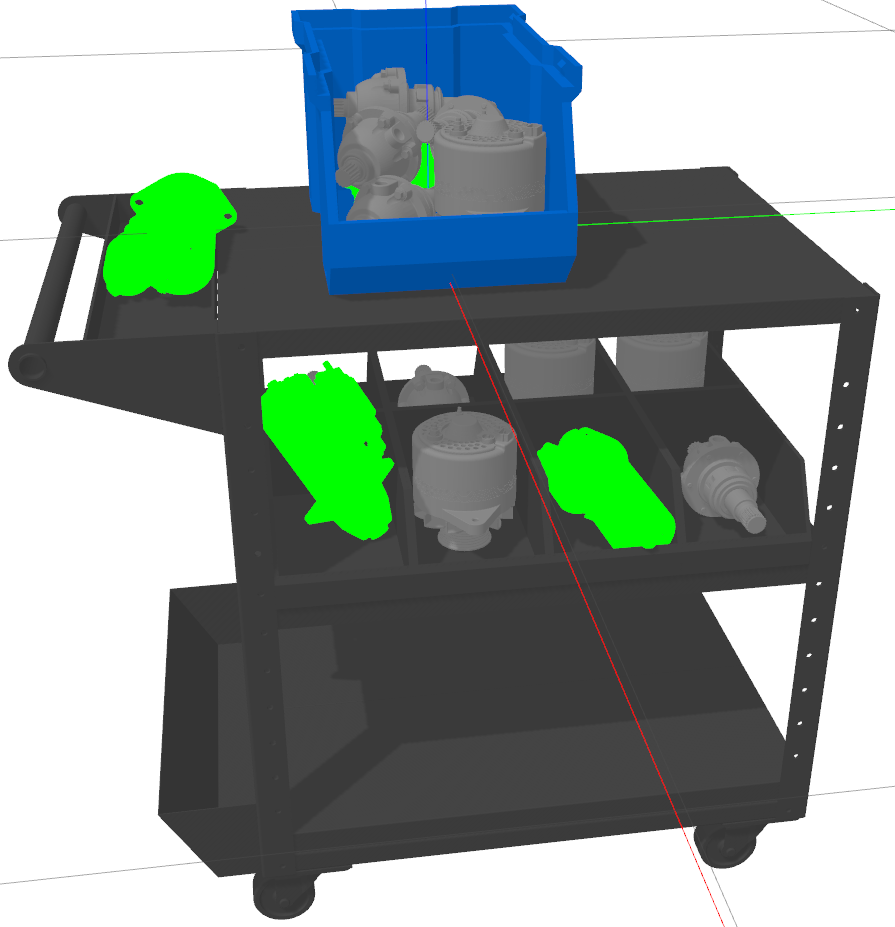
\includegraphics[height=.14\textheight]{sensor-data-processing/multimodel-environment}\hspace{2em}
	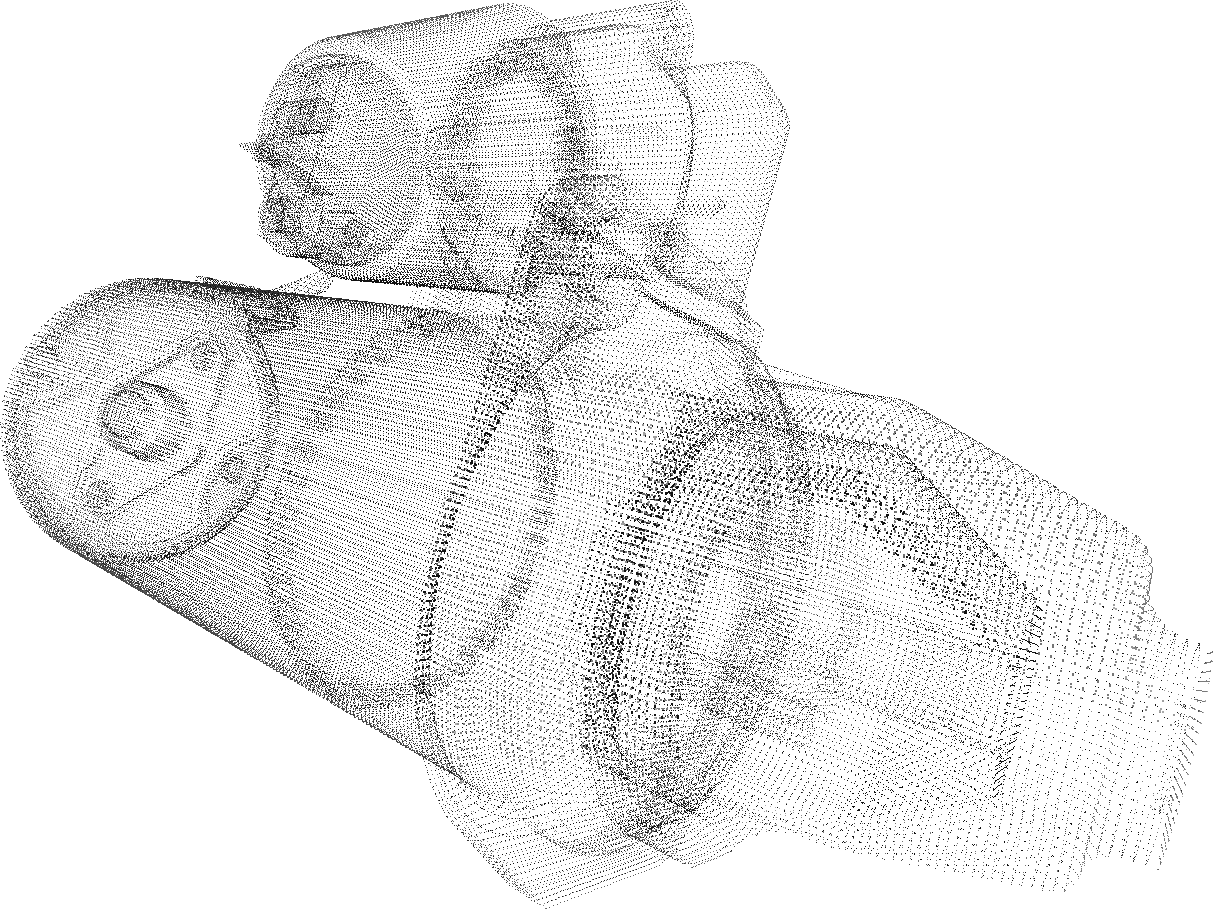
\includegraphics[height=.1\textheight]{sensor-data-processing/cad-model-pointcloud}
	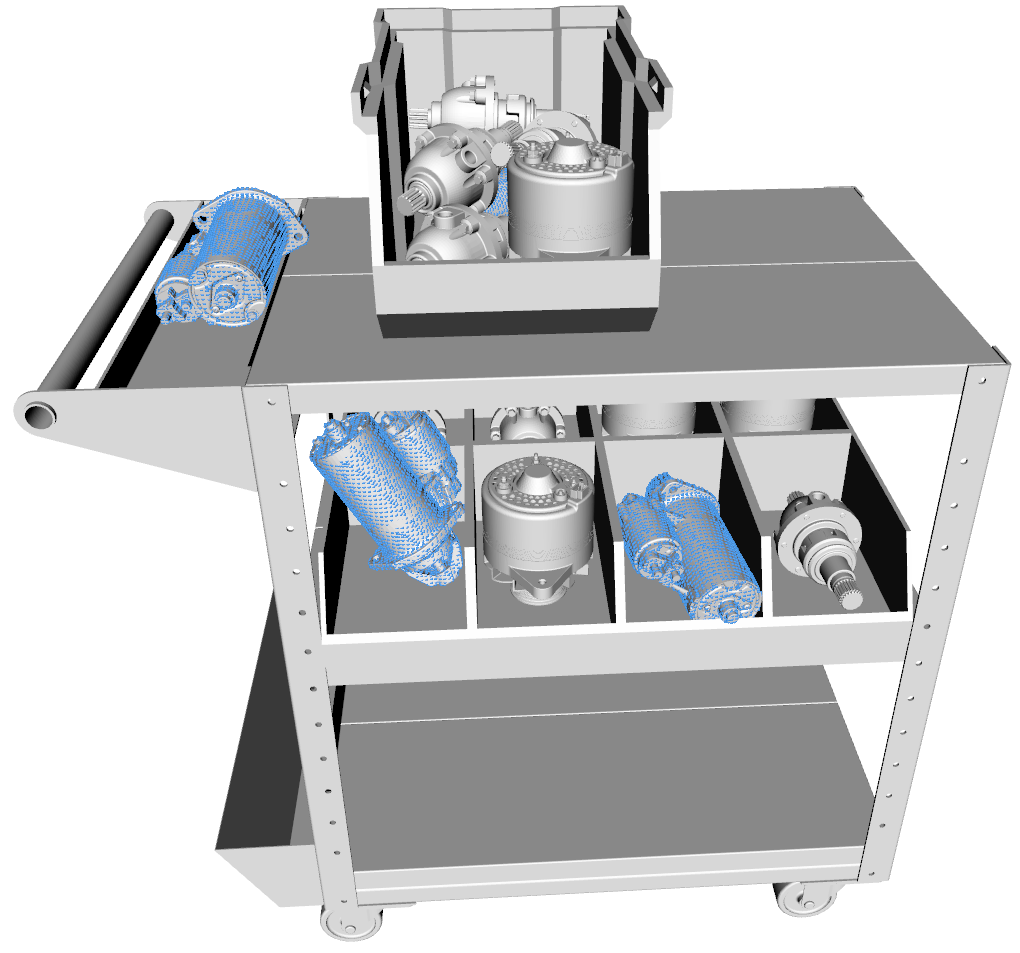
\includegraphics[height=.14\textheight]{sensor-data-processing/multimodel-pointclouds-with-cad}\hspace{2em}
	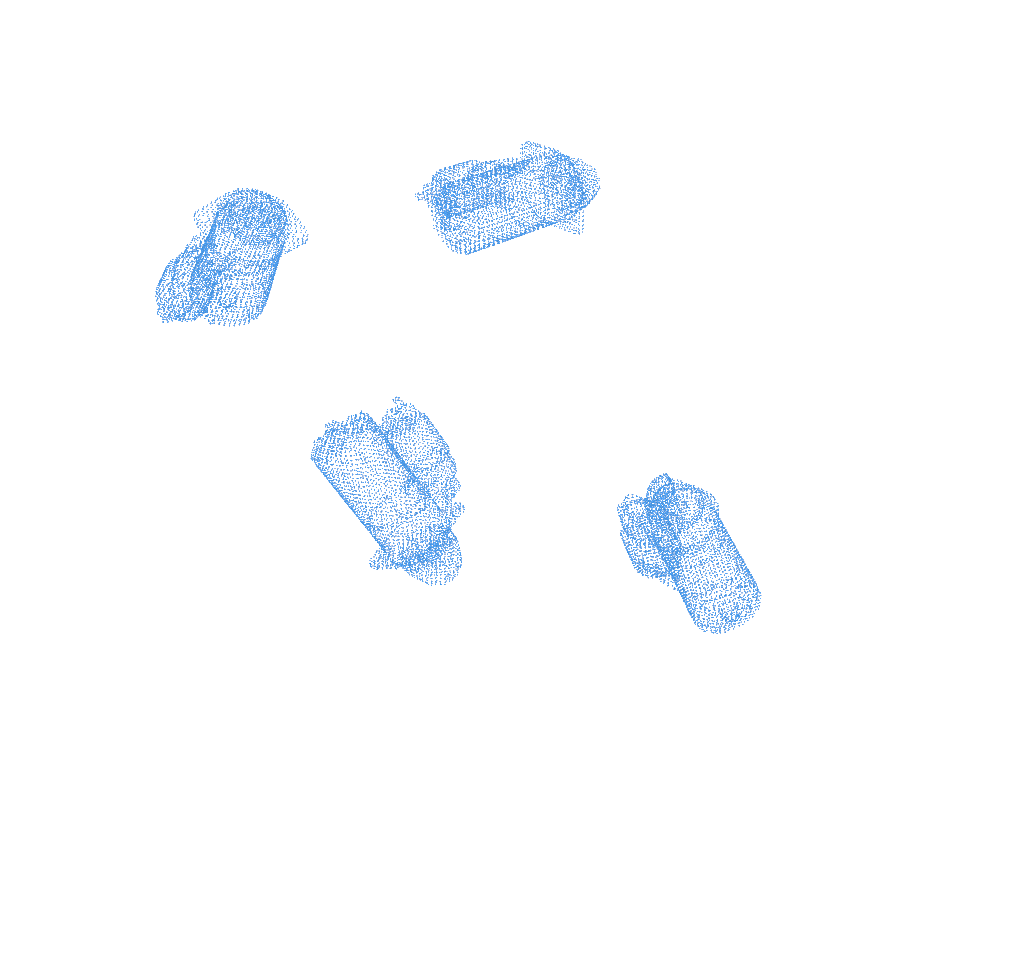
\includegraphics[height=.14\textheight]{sensor-data-processing/multimodel-pointclouds}
	\caption{The first image illustrates the color scene rendering in Gazebo with the target objects in green while the third and fourth images display the reference point cloud that was generated using the CAD point cloud shown on the second image.}
	\label{fig:reference-cloud}
\end{figure}


\subsection{Sensors data analysis}

After loading the simulation world 3D models, deploying the sensors populations on the environment and building the filtered reference point cloud, the proposed system generates a color and depth image for every sensor. Then, for each pixel in the color images that have the target objects unique color, the corresponding pixel in the depth image is retrieved and the 3D point is computed using the pinhole model equations shown in \cref{eq:pointcloud}. Later on, the 3D point is transformed from the sensor coordinate system into the world coordinate system (having all sensor data in the same coordinate system allows fast merging of point clouds from several sensors). After processing all pixels of a given image, the associated point cloud in the world coordinate is filtered with a voxel grid algorithm in order to perform a regular space partition for extracting the centroid of each voxel containing sensor points. This step is critical for allowing consistent evaluation of the object(s) observed surface area percentage, given that sensors with different resolution or at different distances may generate point clouds with different point density even when observing the same surface area. This problem is mitigated by performing a point cloud downsampling using a voxel grid algorithm with a cell size tuned for the objects geometry size we are trying to observe (too many points on a small area for a large object do not provide a significant advantage for 3D perception and require more processing time). Moreover, given that both the reference point cloud and the sensor data point cloud were filtered in the same coordinate frame with the same voxel grid, the surface coverage percentage can be computed very efficiently by simply dividing the number of points in the filtered sensor data point cloud by the number of points in the filtered reference point cloud.

In the end of the sensor analysis stage, each sensor is associated with a filtered point cloud in the world coordinate frame containing only points belonging to the target objects surface.

\footnotesize
\begin{equation}\label{eq:pointcloud}
	\begin{split}
		X = \frac{(PixelCol - XPrincipalPoint) \times PixelDepth}{XFocalLenght}\\
		Y = \frac{(PixelRow - YPrincipalPoint) \times PixelDepth}{YFocalLenght}\\
		Z = PixelDepth
	\end{split}
\end{equation}
\normalsize

\begin{figure}
	\centering
	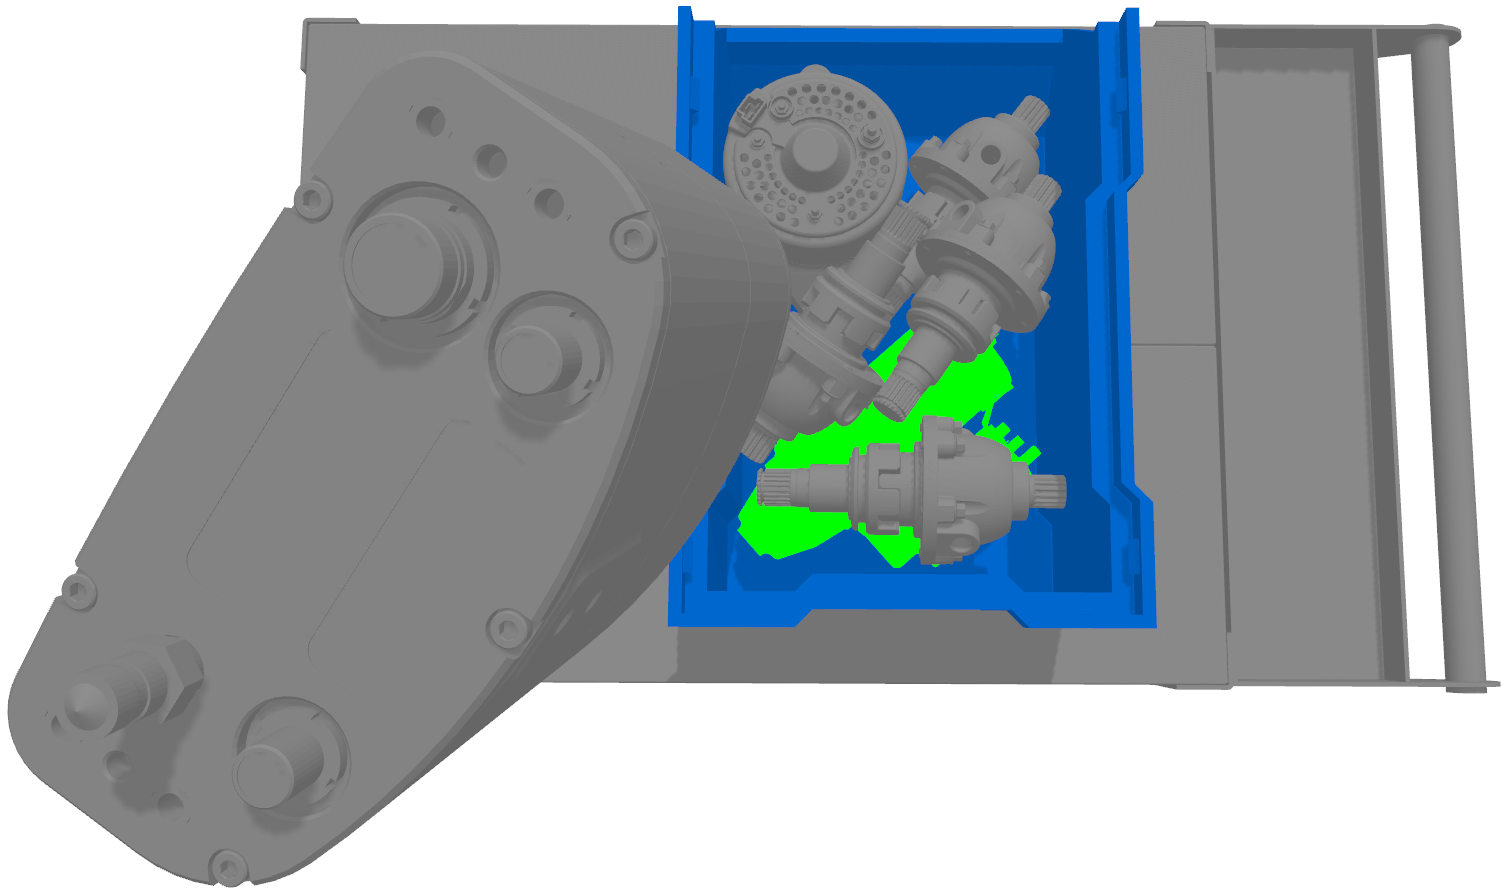
\includegraphics[height=.132\textheight]{sensor-data-processing/sensors-best-view}\\
	\vspace{0.5em}
	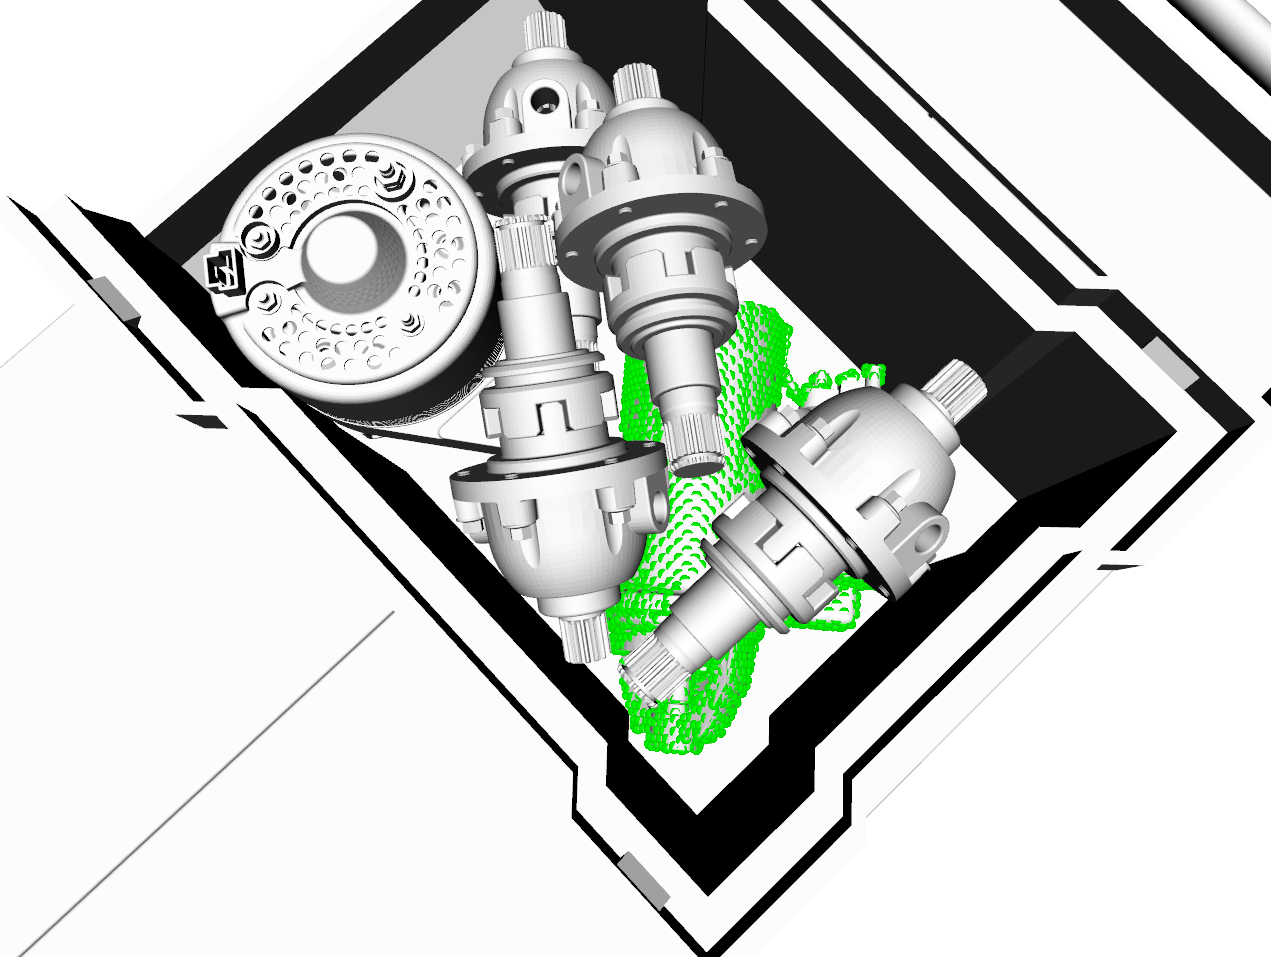
\includegraphics[height=.132\textheight]{sensor-data-processing/rviz-sensor-view}\hspace{2em}
	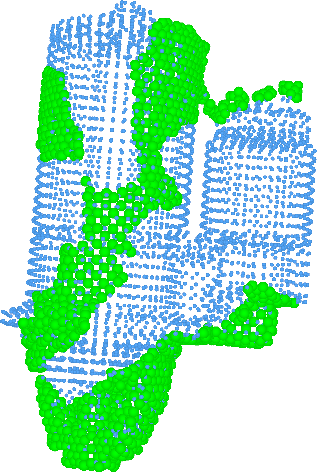
\includegraphics[height=.132\textheight]{sensor-data-processing/rviz-sensor-view-without-cad-with-model}
	\caption{Color image rendered with the Gazebo simulator (top image containing the scene and sensor) along with the generated point cloud for the target object taking into consideration the environment occlusions (bottom images, in which the green spheres are the observed points and the blue spheres are from the filtered point cloud of the associated CAD model).}
\end{figure}


\subsection{Estimation of the best sensors views}

When only one sensor is needed for the task at hand (for example when we are trying to perform active perception of the environment in which the sensor is attached to a robotic arm), the estimation of the best sensor can be performed by simply selecting the one that achieved the best surface coverage percentage. On the other hand, if several sensors are available or we want a single sensor to observe the target objects from a set of N best views, then it is used a \gls{ransac} approach to estimate the constellation of sensors that can achieve the best surface coverage. This approach allows to mitigate and bound the combinatorial explosion that happens when we need to estimate a high number of best views from a large population of sensors. As can be seen in \cref{alg:best-n-views}, this approach runs at most a fixed number of iterations. In each iteration, a set of N sensors are chosen randomly, their sensor data is merged and filtered, and if the surface coverage percentage achieved by this set of views is higher than a given threshold, then the search is stopped. In the end, it is returned the best sensor constellation found along with its associated point could with merged sensor data and the best coverage percentage that was achieved.

\begin{algorithm}[H]
	\caption{Estimation of the best N sensors views}
	\label{alg:best-n-views}
	\begin{algorithmic}[1]
		\State \textbf{Input:}
		\State $N \gets$ number of desired sensors
		\State $P \gets$ point clouds from each deployed sensor
		\State $C \gets$ minimum surface coverage percentage
		\State $I \gets$ maximum number of iterations
		\Procedure{BestSensorsViews}{$N,P,C,I$}
			\State $s \gets Empty$\Comment{best coverage sensors}
			\State $p \gets Empty$\Comment{best merged point cloud}
			\State $c \gets 0$\Comment{best coverage percentage}
			\State $i \gets 0$\Comment{current iteration}
			\While{$i < I$ and $c < C$}
				\State $x \gets SelectSensorsRandomly(P,N)$
				\State $m \gets MergePointClouds(P,x)$
				\State $f \gets FilterPointCloud(m)$
				\State $k \gets ComputeSurfaceCoverage(f)$
				\State $i \gets i + 1$
				\If{$k > c$}
					\State $s \gets x$
					\State $p \gets f$
					\State $c \gets k$
				\EndIf
			\EndWhile
			\State \textbf{return} $(s,p,c)$
		\EndProcedure
	\end{algorithmic}
\end{algorithm}
